\chapter{Evaluation} \label{chap:evaluation}
After explaining the solution's implementation this chapter presents the evaluation's results The evaluation is based on the metrics introduced in section~\ref{sec:fund_loc}.

\section{Accuracy and Precision}
To determine the solution's accuracy and its precision different tests in a real world experiment were performed. For this purpose, the 10 beacons, bought from BEACONinside, were deployed in different parts of the university building. The tests were done in a static environment; thus, the test person was the only dynamic object in the experiment. Besides the deployed beacons, the building is equipped with several WiFi access points, which use the 2.4GHz baseband, too. Thus, their signals may influence the bacons' signals. During the experiments a static particle set size of 200~particles was used, as mentioned in chapter~\ref{chap:pf}.

\subsection*{Experiment~1}
For the first experiment only one lecture hall was equipped with all 10 beacons. Figure~\ref{fig:f007} shows a picture of the lecture hall for illustration purposes. On the following screenshots the lecture hall is depicted on the map's lower part. The picture was taken from the hall's lower left corner.

\begin{figure}
	\includegraphics[width=0.9\textwidth]{figures/F007}
	\caption{Shows the lecture hall depicted on the map's lower part.}
	\label{fig:f007}
\end{figure}

\begin{figure}
	\subfloat[Path] {
  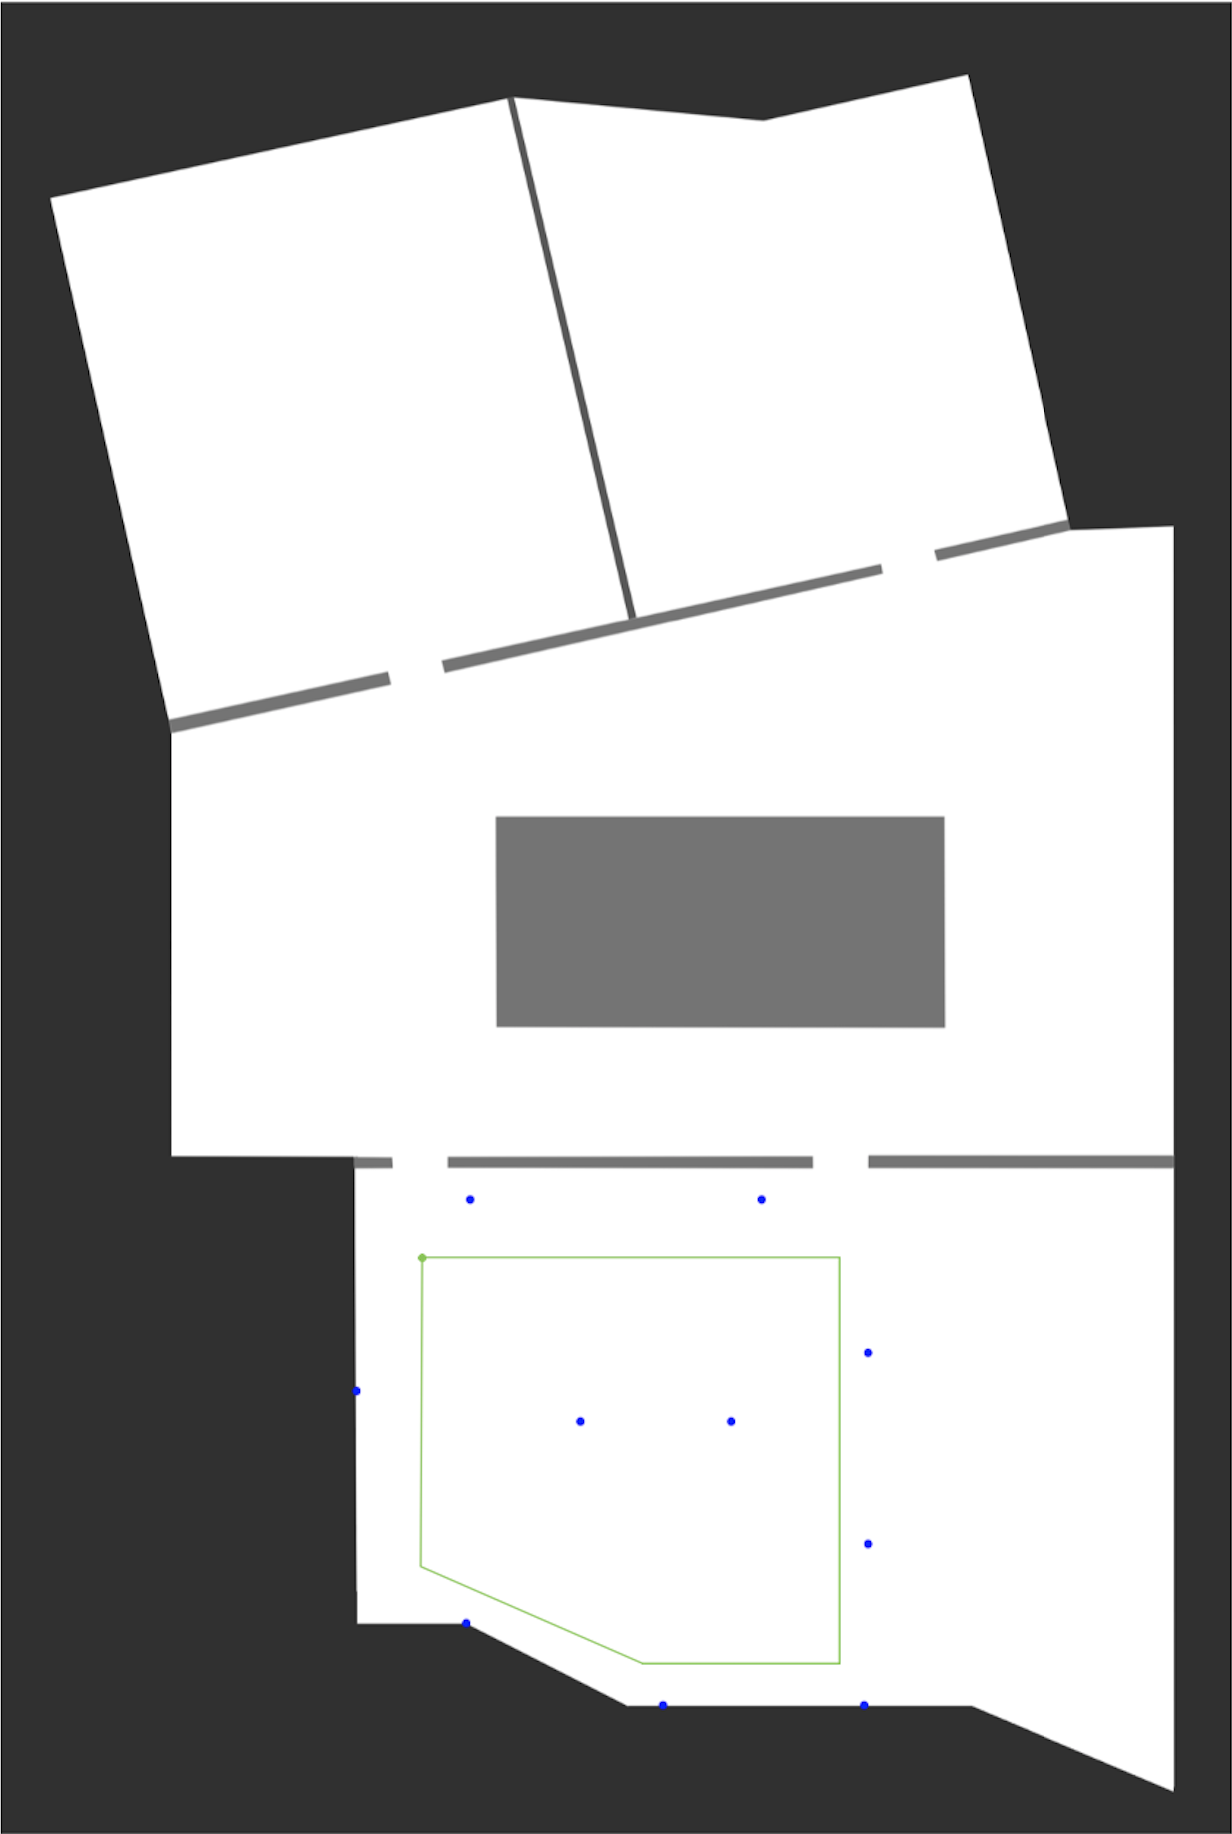
\includegraphics[height=0.4\textheight]{figures/eval_1_path}
  \label{fig:exp1_path}
}
\subfloat[] {
  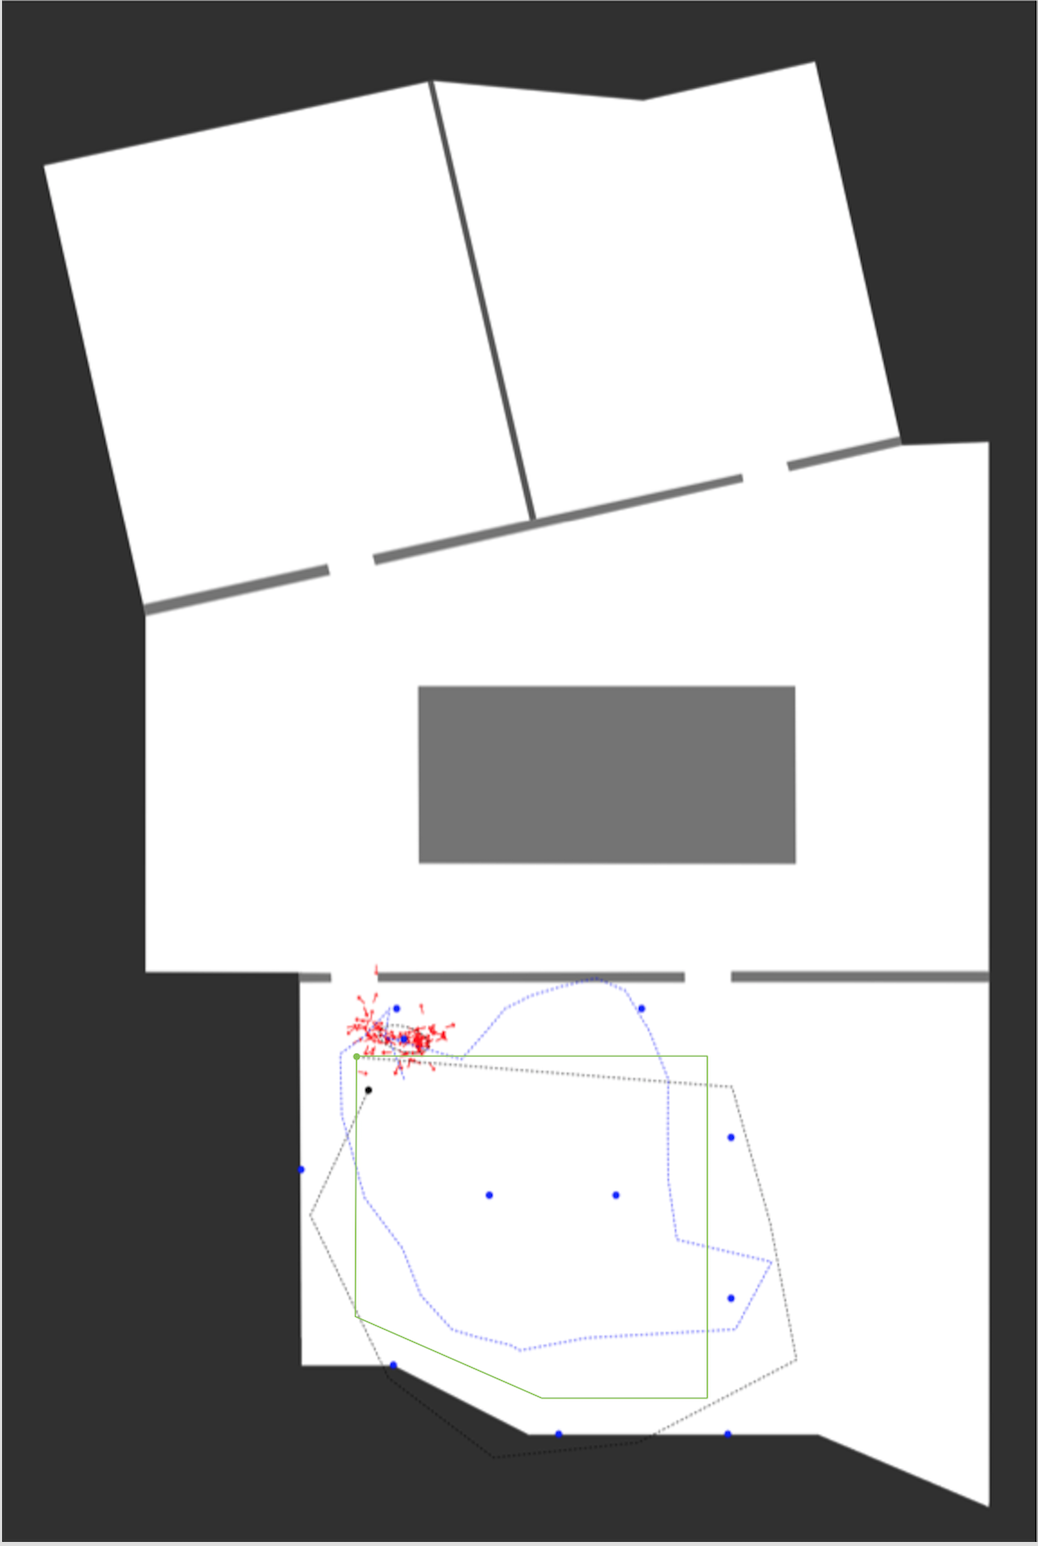
\includegraphics[height=0.4\textheight]{figures/eval_1_1}
  \label{fig:exp1_img_1}
}

\subfloat[] {
  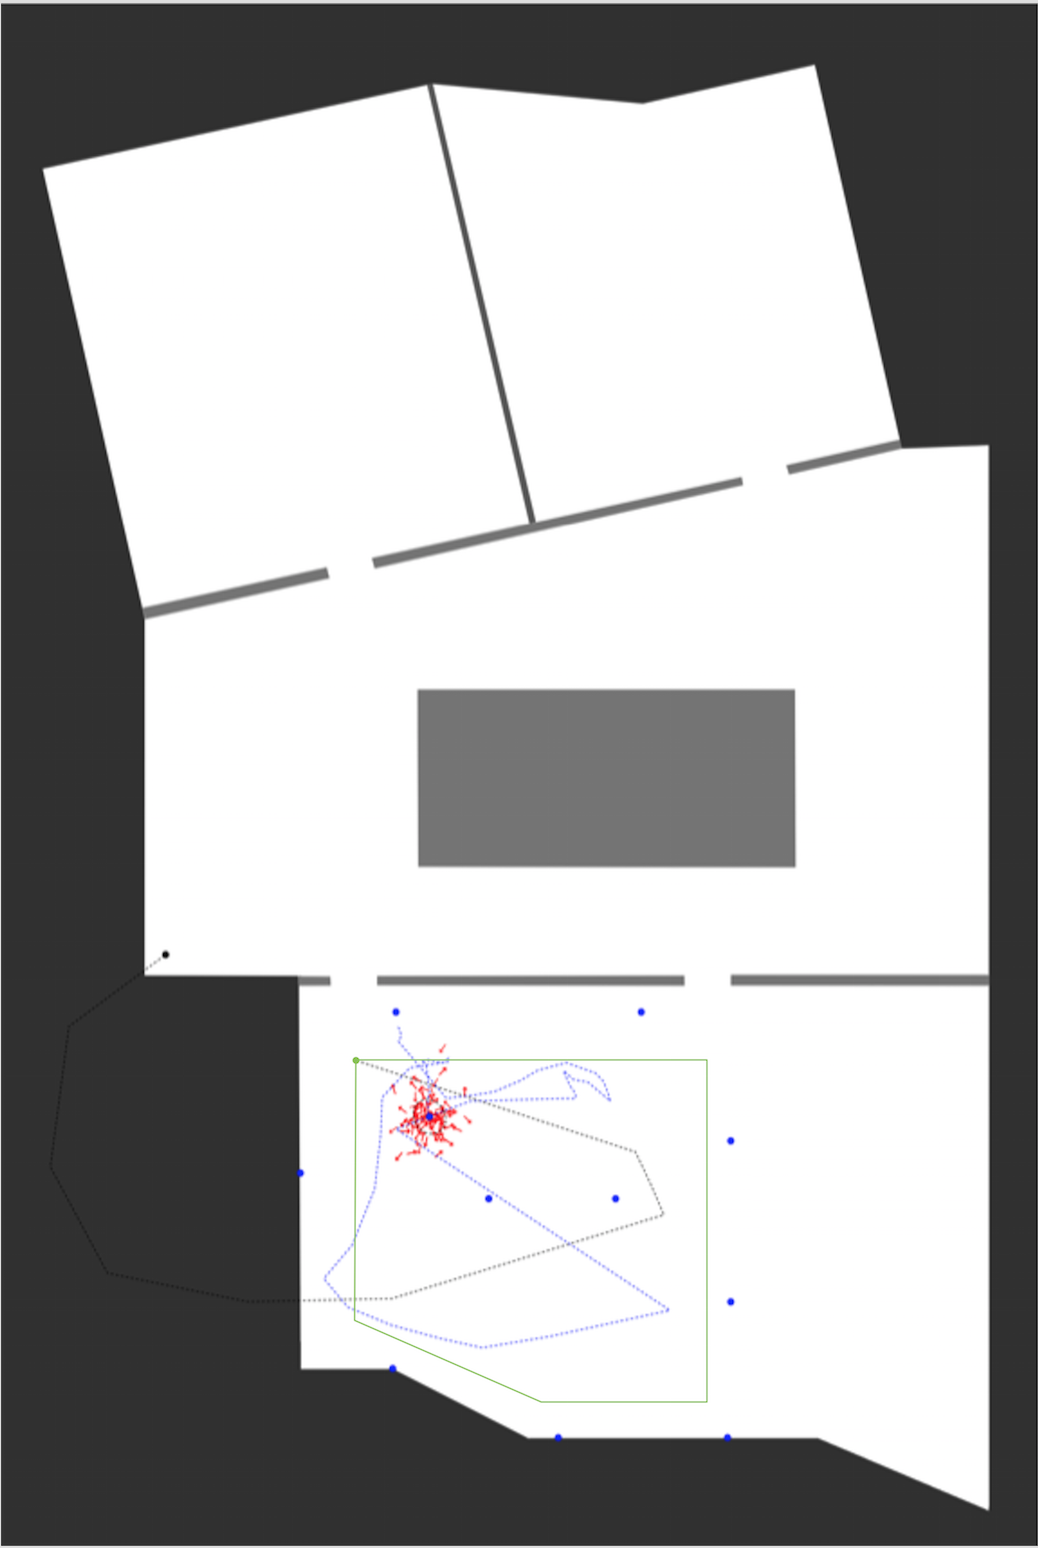
\includegraphics[height=0.4\textheight]{figures/eval_1_2}
  \label{fig:exp1_img_2}
}
\subfloat[] {
  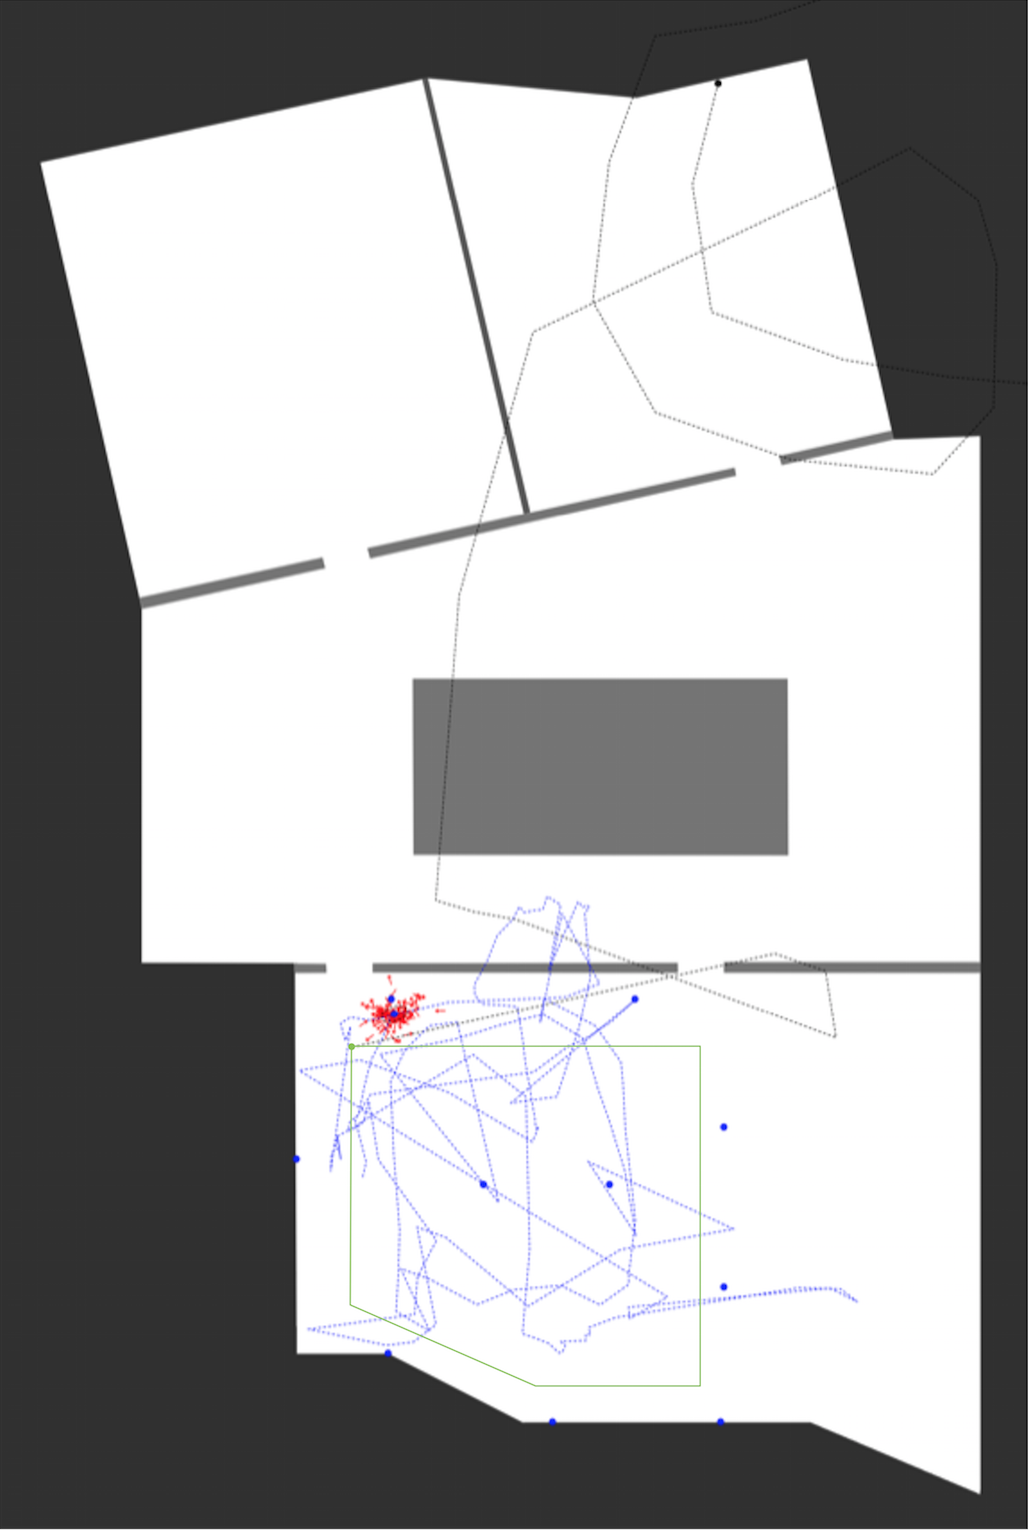
\includegraphics[height=0.4\textheight]{figures/eval_1_3}
  \label{fig:exp1_img_3}
}

	\caption{The Screenshots illustrate results of Experiment~1.}
	\label{fig:exp1_screenshot}
\end{figure}

The purpose of this experiment is to test how good the localization works inside the shown lecture hall. The lecture hall, depicted in the lower part of figure~\ref{fig:exp1_path}, is  $\approx$\,15\,m long and 8\,-–\,11\,m wide. The beacons' positions are depicted as blue circles.

To determine the algorithms accuracy, the test person walked on a specified path, depicted in green, beginning and ending at the upper left corner. At the end of each walk the application's estimated end position is compared with the true end position by calculating the error in form of the euclidian distance. As mentioned in section~\ref{sec:algo_locEstimation}, the location can be estimated by either calculating the mean of $\chi$, or by calculating its weighted mean. To be able to compare them the error of both approaches is calculated.

Additionally, the error of the motion tracking's end position is compared with the true position. To be able to compare the motion error with the estimated location error by taking into account the motion drift, the experiment was divided into three scenarios. First, the test person walked just one round on the green path. Second, two rounds, and third three rounds. For each scenario the test user walks three times in clockwise and three times in counter-clockwise direction on the path.

Furthermore, this experiment is used to determine if the accuracy improves after being stationary at the end position for a short time. Thus, two location errors are determined. The error of the estimated position directly after integrating the last reported motion and the location error $\approx$\,5\,s later.


\begin{table}
	\subfloat[Error at stop]{
  \begin{tabular}{c||cc|cc}
    Scenario & $\mu$ & $\sigma$ & $\mu_w$ & $\sigma_w$\\
    \hline
    1 & 2.23 & 2.74 & 2.08 & 2.55\\
    2 & 2.16 & 2.53 & 2.16 & 2.53\\
    3 & 3.00 & 3.64 & 3.55 & 4.23\\
    \hline
    1--3 & 2.47 & 2.83 & 2.60 & 3.01\\
  \end{tabular}
  \label{tab:evaluationResultExp1_1}
}
\subfloat[Error after being $\approx$\,5\,s stationary]{
  \begin{tabular}{c||cc|cc}
    Scenario & $\mu$ & $\sigma$ & $\mu_w$ & $\sigma_w$\\
    \hline
    1 & 2.19 & 3.13 & 2.17 & 3.13\\
    2 & 1.94 & 2.52 & 1.95 & 2.53\\
    3 & 2.73 & 3.71 & 2.74 & 3.72\\
    \hline
    1--3 & 2.29 & 2.97 & 2.29 & 2.97\\
  \end{tabular}
  \label{tab:evaluationResultExp1_2}
}

\subfloat[Motion Tracking Error]{
  \begin{tabular}{c||cc}
    Scenario & $\mu$ & $\sigma$\\
    \hline
    1 & 3.63 & 4.24\\
    2 & 7.11 & 8.05\\
    3 & 10.81 & 13.21\\
    \hline
    1--3 & 7.19 & 13.21\\
  \end{tabular}
  \label{tab:evaluationResultExp1_3}
}

	\caption{Depicts the results of experiment~1.}
	\label{tab:evaluationResultExp1}
\end{table}

\begin{figure}
	\begin{tikzpicture}
  \begin{axis}[trim axis left, trim axis right, height=0.4\textheight,
    xlabel={Scenario},
    ylabel={Error (m)},
    legend entries={$\mu$ (tab.\ \ref{tab:evaluationResultExp1_1}), $\mu_w$ (tab.\ \ref{tab:evaluationResultExp1_1}), $\mu$ (tab.\ \ref{tab:evaluationResultExp1_2}), $\mu_w$ (tab.\ \ref{tab:evaluationResultExp1_2}), $\mu$ (tab.\ \ref{tab:evaluationResultExp1_3})},
    legend pos=north west,
    grid = major,
    xtick=data]
    \addplot [blue, only marks] table[col sep=semicolon, x=scenario, y=mean] {csv/eval/Eval_1_ep1/NDFScenario.csv};
    \addplot [blue, only marks, mark=square*] table[col sep=semicolon, x=scenario, y=w_mean] {csv/eval/Eval_1_ep1/NDFScenario.csv};
    \addplot [red, only marks] table[col sep=semicolon, x=scenario, y=mean] {csv/eval/Eval_1_ep2/NDFScenario.csv};
    \addplot [red, only marks, mark=square*] table[col sep=semicolon, x=scenario, y=w_mean] {csv/eval/Eval_1_ep2/NDFScenario.csv};
    \addplot [green, only marks] table[col sep=semicolon, x=scenario, y=mean] {csv/eval/Eval_1_motion/NDFScenario.csv};
  \end{axis}
\end{tikzpicture}

	\caption{Visualizes the results shown in table~\ref{tab:evaluationResultExp1}.}
	\label{fig:exp1_visualization}
\end{figure}

\subsubsection*{Results}
The results are shown in table~\ref{tab:evaluationResultExp1} and are visualized in figure~\ref{fig:exp1_visualization}.

Table~\ref{tab:evaluationResultExp1_1} depicts the average distance error and the error's distribution, for each scenario, directly after integrating the last motion. Table~\ref{tab:evaluationResultExp1_2} shows the determined values recorded $\approx$\,5\,s after the last motion integration. The calculated average error using $\chi$'s mean as location is denoted with $\mu$. The errors standard deviation is denoted with $\sigma$. $\mu_w$ and $\sigma_w$ are the average error and its standard deviation using the weighted mean of $\chi$ for the position estimation.
Table~\ref{tab:evaluationResultExp1_3} shows the motion tracking's error $\mu$ and the error's distribution in form of its standard deviation $\sigma$.

The results show that during the experiment an accuracy of 2.29\,m\,--\,2.6\,m is achieved. It also shows that the location estimation tends to improve after being stationary at the end position, as expected.

The difference between the two position estimation approaches is very small. The result sways, sometimes $\chi$'s mean, and sometimes its weighted mean is more accurate. Supposedly the minimal difference is based on the particle cloud's high concentration.

The result's visualization also clearly shows that the motion error grows with increasing number of rounds, whereas the estimated position error only grows minimally. Supposedly, the minimally higher error is the result of a few outliers in the motion error, which of course affects the position estimation. Besides the path, figure~\ref{fig:exp1_screenshot} depicts three examples of the experiment. They clearly show, that the motions' accuracy influences the position estimation. If the motion is completely wrong (fig.\ \ref{fig:exp1_img_3}), the in section~\ref{sec:algo_stationary} introduced recovery feature often needs to intervene, which causes several jumps in the position estimation. Whereas figure~\ref{fig:exp1_img_2} shows, that if the motion is acceptably wrong, the algorithm can correct the path (of course not perfectly). If the motion estimation fits the true path the estimated path depends just on the beacons' signal quality, as shown in figure~\ref{fig:exp1_img_1}.

\subsection*{Experiment~2}
The purpose of the second experiment is on one hand, to double check the implementation's accuracy by using another position, and on the other hand, to demonstrate the dependency of the estimation's accuracy and the amount of deployed beacons.

This time the test person walked on a random path. The person started at the orange circle, shown in figure~\ref{fig:exp2_imgs} on the upper left corner, and stopped at the green circle, approximately in the figure's center.

To demonstrate the impact of reducing the number of deployed beacons, five test walks with all 10\,beacons deployed were recorded first. Then the simulation was used to play back the recorded values by reducing the input to a lower number of deployed beacons. Thus, the values are directly comparable, because for all test cases the exact same input data is used. Also for this experiment the location error is calculated directly after integrating the last motion and $\approx$\,5\,s later.

\subsubsection*{Results}
The experiment's results are shown in table~\ref{tab:evaluationResultExp2} and visualized in figure~\ref{fig:exp2_visualization}. The corresponding beacon deployment is shown in figure~\ref{fig:exp2_imgs}.

First of all, the result clearly shows that the difference between $\chi$'s mean and its weighted mean is negligible.

Secondly, it clearly shows that the estimated location compared to the motion is more accurate. Additionally, it depicts that the location estimation drastically improves after being stationary, for some seconds, i.e.\ for $\approx$\,5\,s.

The result also indicates that the estimation's accuracy depends on the deployed number of beacons. Thus, the more beacons, the less error in the position estimation. But it also shows, that at a certain beacon density the error's reduction converges. Furthermore, deploying more beacons does not always improve accuracy. This seems to be the case in the experiment by reducing the beacon amount from four to two deployed beacons. Supposedly, the signals of the two removed beacons were too bad, and thus produced a worse estimation result.

\begin{table}
	\subfloat[Error at stop] {
  \begin{tabular}{c||cc|cc}
    Beacons & $\mu$ & $\sigma$ & $\mu_w$ & $\sigma_w$\\
    \hline
    10 & 3.38 & 4.04 & 3.33 & 3.99\\
    8 & 3.18 & 3.94 & 3.15 & 3.91\\
    6 & 4.39 & 5.72 & 4.37 & 5.70\\
    4 & 4.48 & 5.28 & 4.50 & 5.30\\
    2 & 3.68 & 4.63 & 3.69 & 4.66\\
  \end{tabular}
  \label{tab:evaluationResultExp2_1}
}
\subfloat[Error after $\approx 5~sec$] {
  \begin{tabular}{c||cc|cc}
    Beacons & $\mu$ & $\sigma$ & $\mu_w$ & $\sigma_w$\\
    \hline
    10 & 1.52 & 1.80 & 1.52 & 1.79\\
    8 & 1.67 & 2.07 & 1.67 & 2.06\\
    6 & 2.87 & 3.96 & 2.89 & 3.96\\
    4 & 3.23 & 3.88 & 3.23 & 3.88\\
    2 & 2.95 & 3.60 & 2.98 & 3.63\\
  \end{tabular}
  \label{tab:evaluationResultExp2_2}
}

\subfloat[Error of motion tracking]{
  \begin{tabular}{c||cc}
    Beacons & $\mu$ & $\sigma$\\
    \hline
    2--10 & 5.68 & 7.04
  \end{tabular}
  \label{tab:evaluationResultExp2_3}
}

	\caption{Depicts the results of experiment~2.}
	\label{tab:evaluationResultExp2}
\end{table}

\begin{figure}
	\begin{tikzpicture}
  \begin{axis}[trim axis left, trim axis right, height=0.35\textheight,
    xlabel={Deployed Beacon Count},
    ylabel={Error (m)},
    legend entries={$\mu$ (Table \ref{tab:evaluationResultExp2_1}), $\mu_w$ (Table \ref{tab:evaluationResultExp2_1}), $\mu$ (Table \ref{tab:evaluationResultExp2_2}), $\mu_w$ (Table \ref{tab:evaluationResultExp2_2}), $\mu$ (Table \ref{tab:evaluationResultExp2_3})},
    legend pos=south east,
    grid = major,
    xtick=data, x dir=reverse]
    \addplot [blue, only marks] table[col sep=semicolon, x=beacon, y=mean] {csv/eval/Eval_2_ep1/NDFBeacon.csv};
    \addplot [blue, only marks, mark=square*] table[col sep=semicolon, x=beacon, y=w_mean] {csv/eval/Eval_2_ep1/NDFBeacon.csv};
    \addplot [red, only marks] table[col sep=semicolon, x=beacon, y=mean] {csv/eval/Eval_2_ep2/NDFBeacon.csv};
    \addplot [red, only marks, mark=square*] table[col sep=semicolon, x=beacon, y=w_mean] {csv/eval/Eval_2_ep2/NDFBeacon.csv};
    \addplot [green, only marks] table[col sep=semicolon, x=beacon, y=mean] {csv/eval/Eval_2_motion/NDF.csv};
  \end{axis}
\end{tikzpicture}

	\caption{Visualizes the results shown in table~\ref{tab:evaluationResultExp2}.}
	\label{fig:exp2_visualization}
\end{figure}


\begin{figure}
	\subfloat[10 Beacons] {
  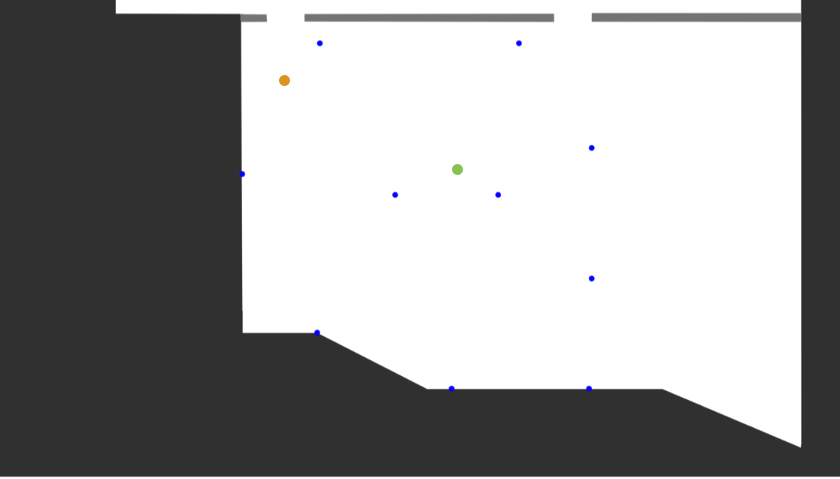
\includegraphics[width=0.45\textwidth]{figures/eval_2_10B}
}
\subfloat[8 Beacons] {
  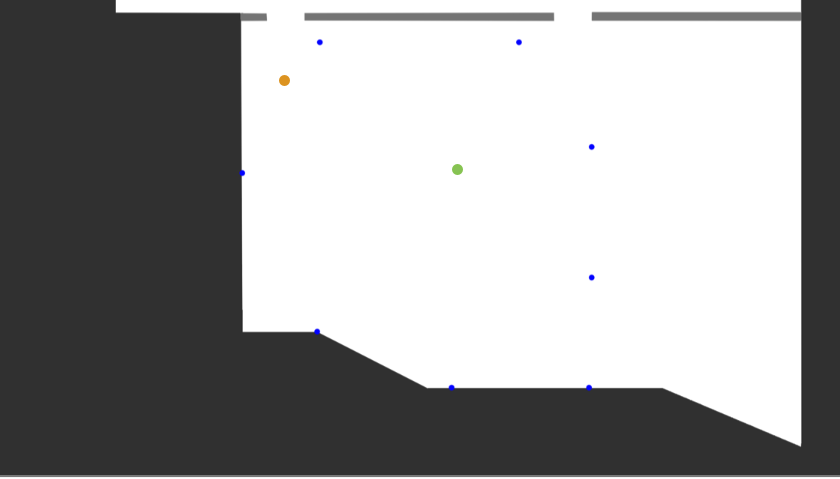
\includegraphics[width=0.45\textwidth]{figures/eval_2_8B}
}

\subfloat[6 Beacons] {
  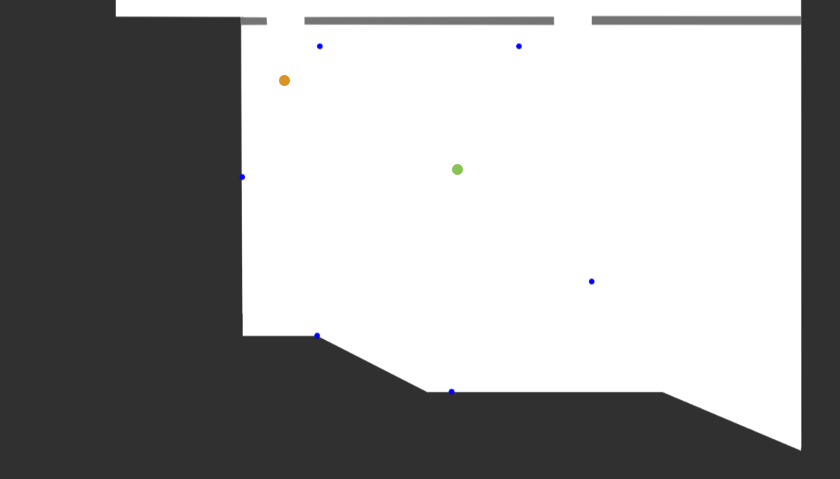
\includegraphics[width=0.45\textwidth]{figures/eval_2_6B}
}
\subfloat[4 Beacons] {
  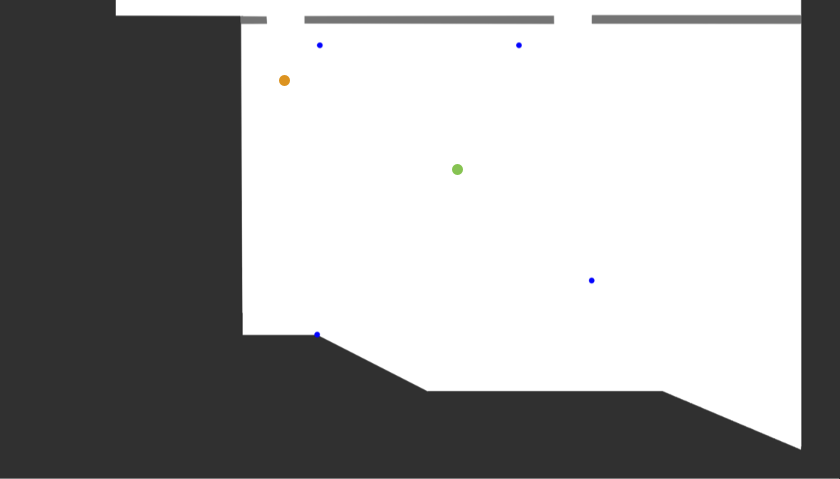
\includegraphics[width=0.45\textwidth]{figures/eval_2_4B}
}

\subfloat[2 Beacons] {
  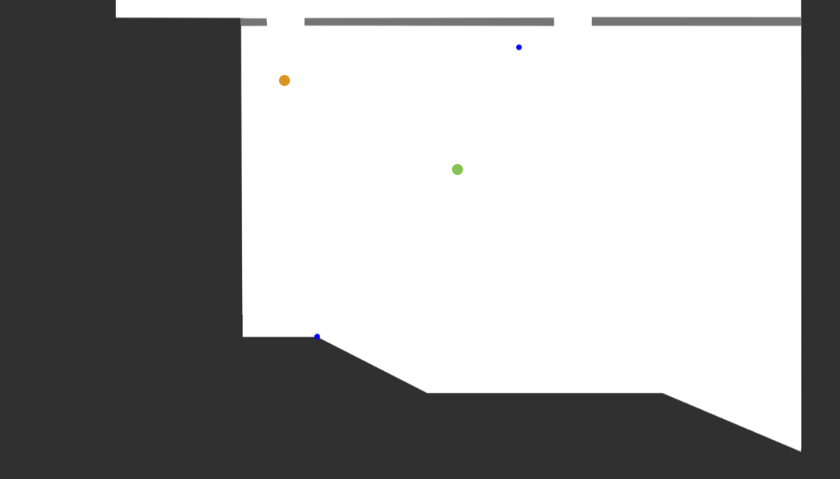
\includegraphics[width=0.45\textwidth]{figures/eval_2_2B}
}

	\caption{Shows the different beacon deployments during the experiment.}
	\label{fig:exp2_imgs}
\end{figure}


\subsection*{Experiment~3}
After evaluating the solution's accuracy in the first two experiments, this experiment shows how good the solution is able to track a users path in a larger scenario. Hence, the buildings foyer, depicted in figure~\ref{fig:f-foyer}, and one / two lecture halls were additionally used. For the experiments, only 10\,beacons were used, as shown on the maps. The map depicts an actual space of $\approx$\,22.22\,m\,$\times$\,33.06\,m.

The first example is depicted in figure~\ref{fig:exp3_imgs}. The green line approximates the actual path, beginning at the top right. The black dashed line shows the motion path, which is just the combination of pedometer and heading. The estimated path is marked as a blue dashed line. Figure~\ref{fig:exp3_imgs_1} shows an example where the motion was very accurate, actually more accurate than the estimated path. Whereas, Figure~\ref{fig:exp3_imgs_2}, \ref{fig:exp3_imgs_3}, and~\ref{fig:exp3_imgs_4} depict examples, where the motion path is bad or completely wrong, but the algorithm was more or less able to approximate the actual path.

Figure~\ref{fig:exp3_imgs_5} depicts another example, where the test person walked around the big stairs in the middle of the building's foyer. The screenshot shows, that the algorithm was able to approximate this path as well. During this example the foyer was equipped with only 4\,beacons as shown on the map. But, the experiment also showes that 4\,beacons are not sufficient for such a large area if the motion is incorrect.

Another example path is shown in figure~\ref{fig:exp3_imgs_6}. During this example the wall between the two upper halls was opened. As shown, the algorithm was able to track the path. But usually this would not be possible without having such an accurate motion, even by using 10\,beacons. Furthermore, the screenshot shows that the estimated end position is actually not at the true position, but rather $\approx$\,4\,--\,5\,m too distant. The screenshot shows that two particles are located next to the true position, and that the plotted $\sigma-\text{ellipse}$ is oriented towards these two particles. The reason for that is, that the algorithms weight sum dropped below the recovery's threshold, and thus the recovery feature was executed. Unfortunately, the data recording was stopped at this point in time, otherwise it is very likely that the particle cloud would have jumped to the true location where the two particles were already located. 


\begin{figure}
	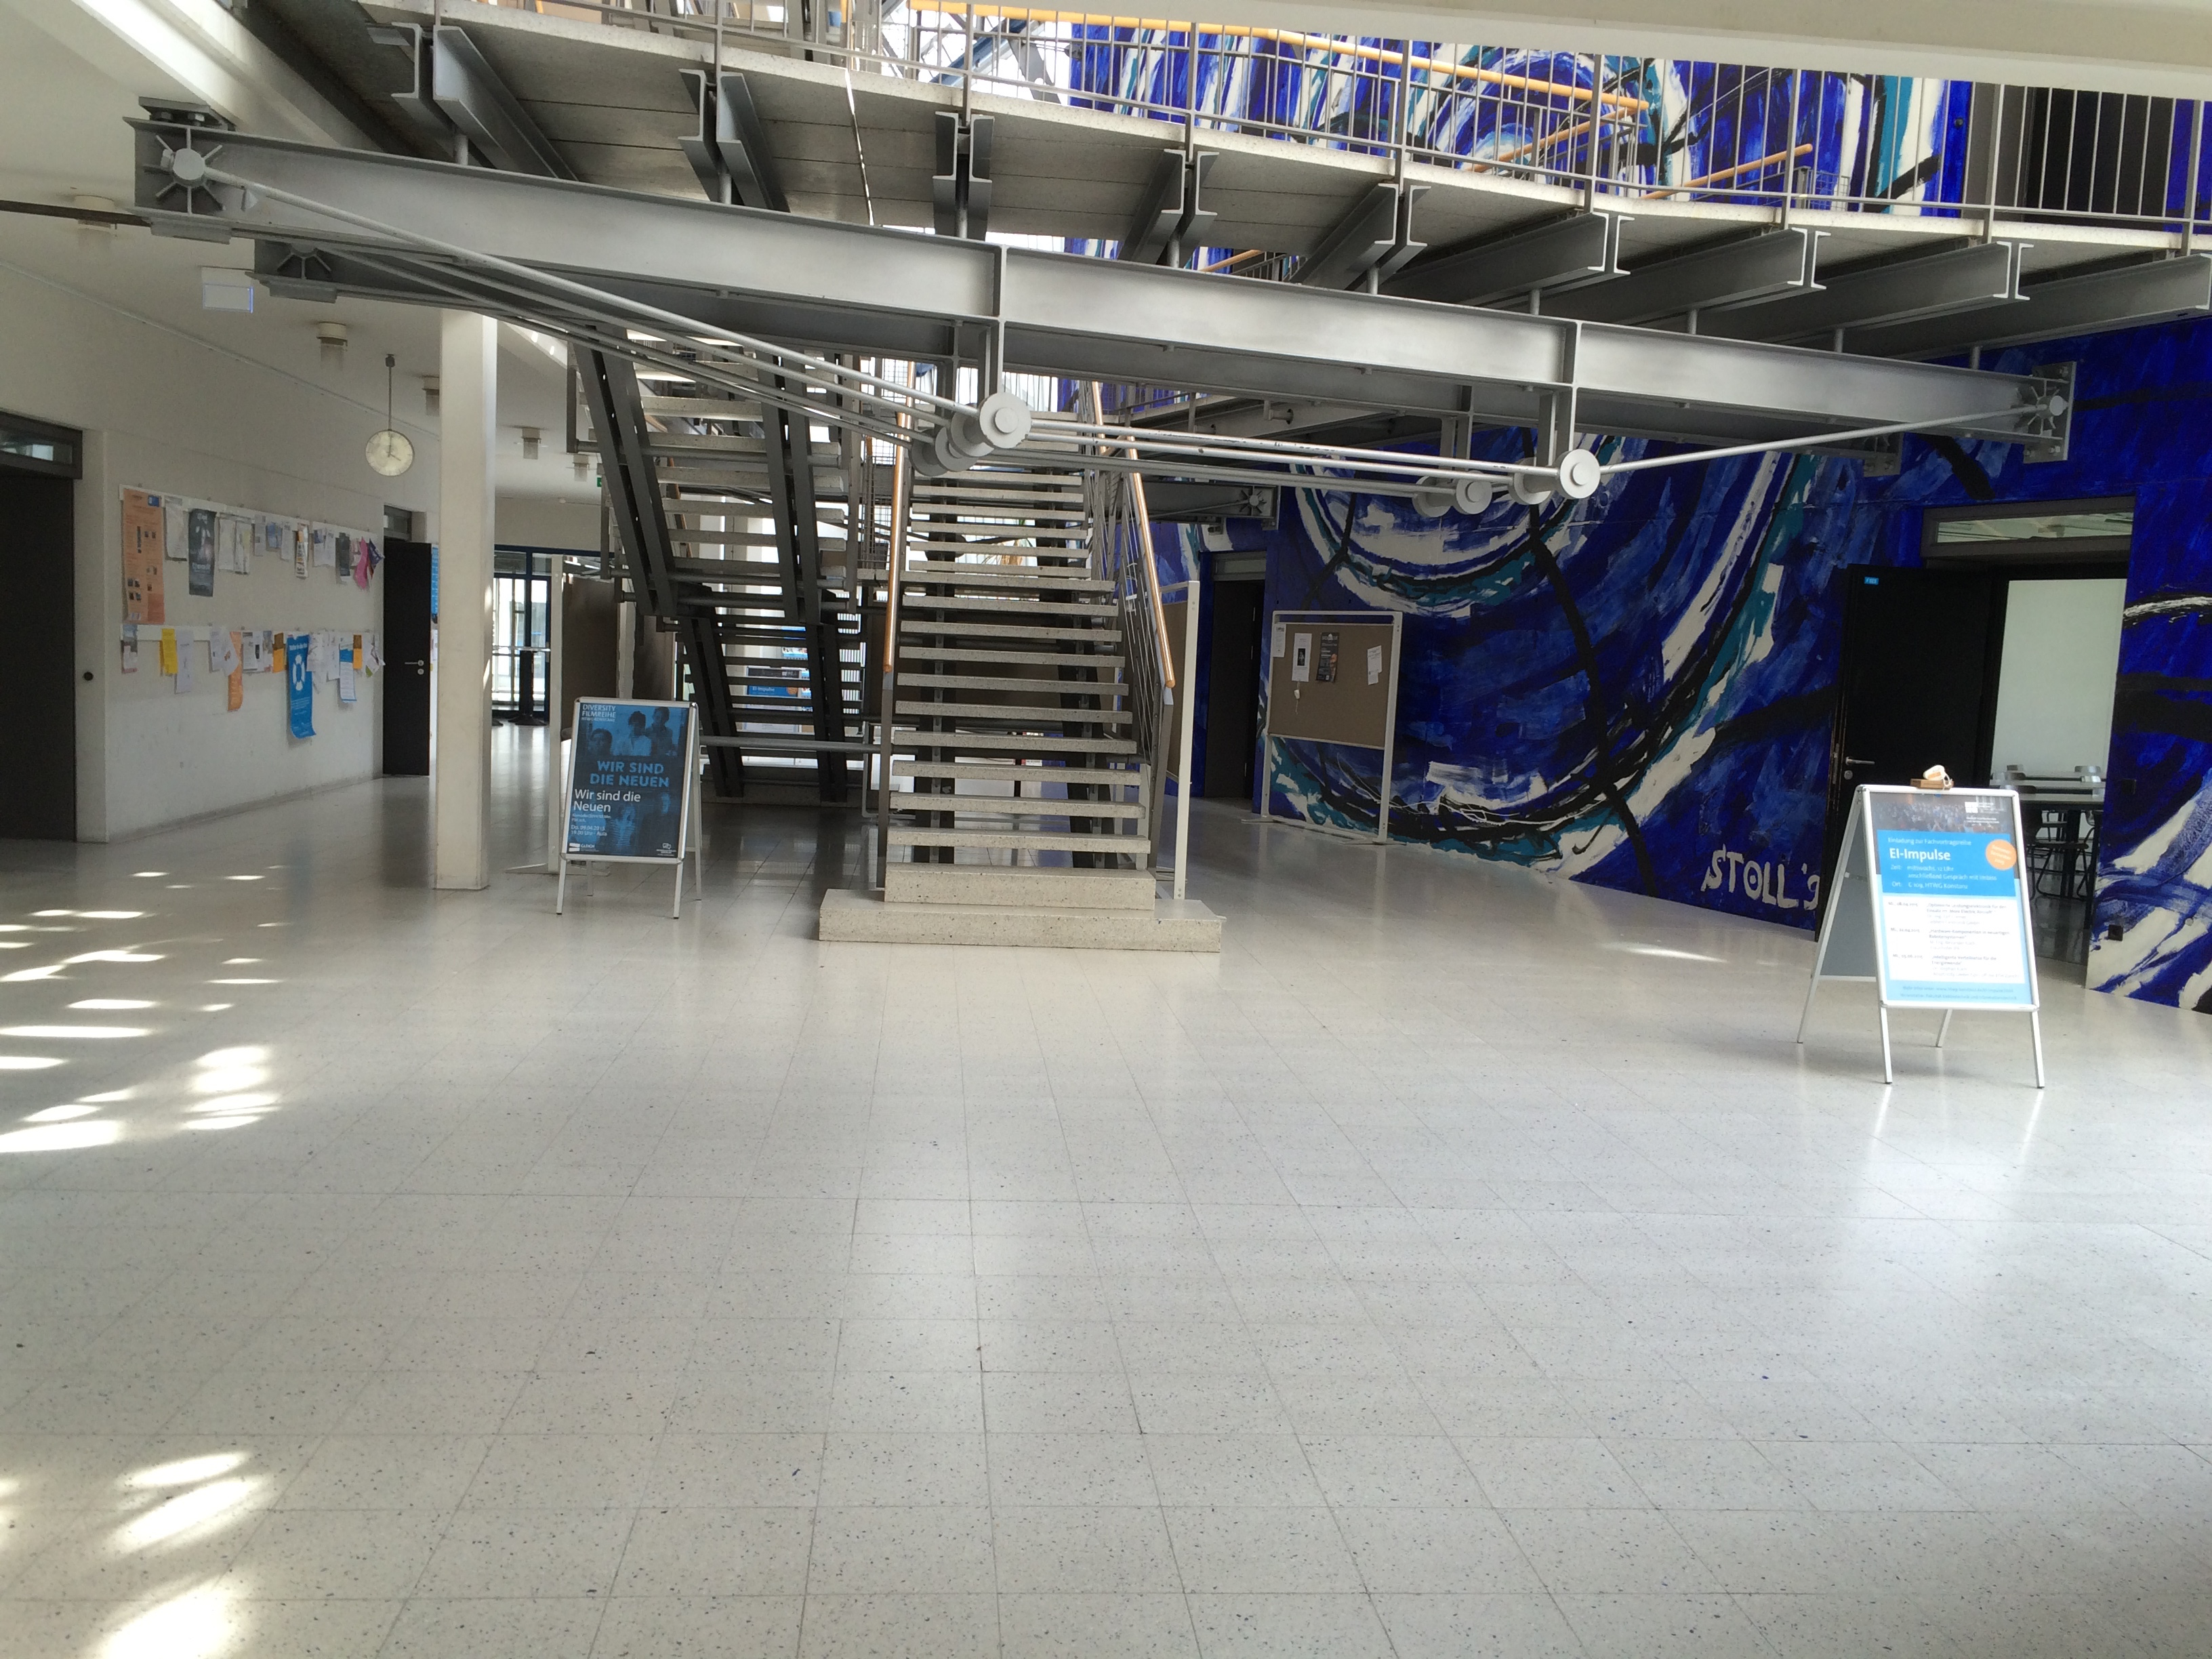
\includegraphics[width=0.9\textwidth]{figures/F-Foyer}
	\caption{Shows the buildings Foyer depicted on the map's middle.}
	\label{fig:f-foyer}
\end{figure}

\begin{figure}
	\subfloat[] {
  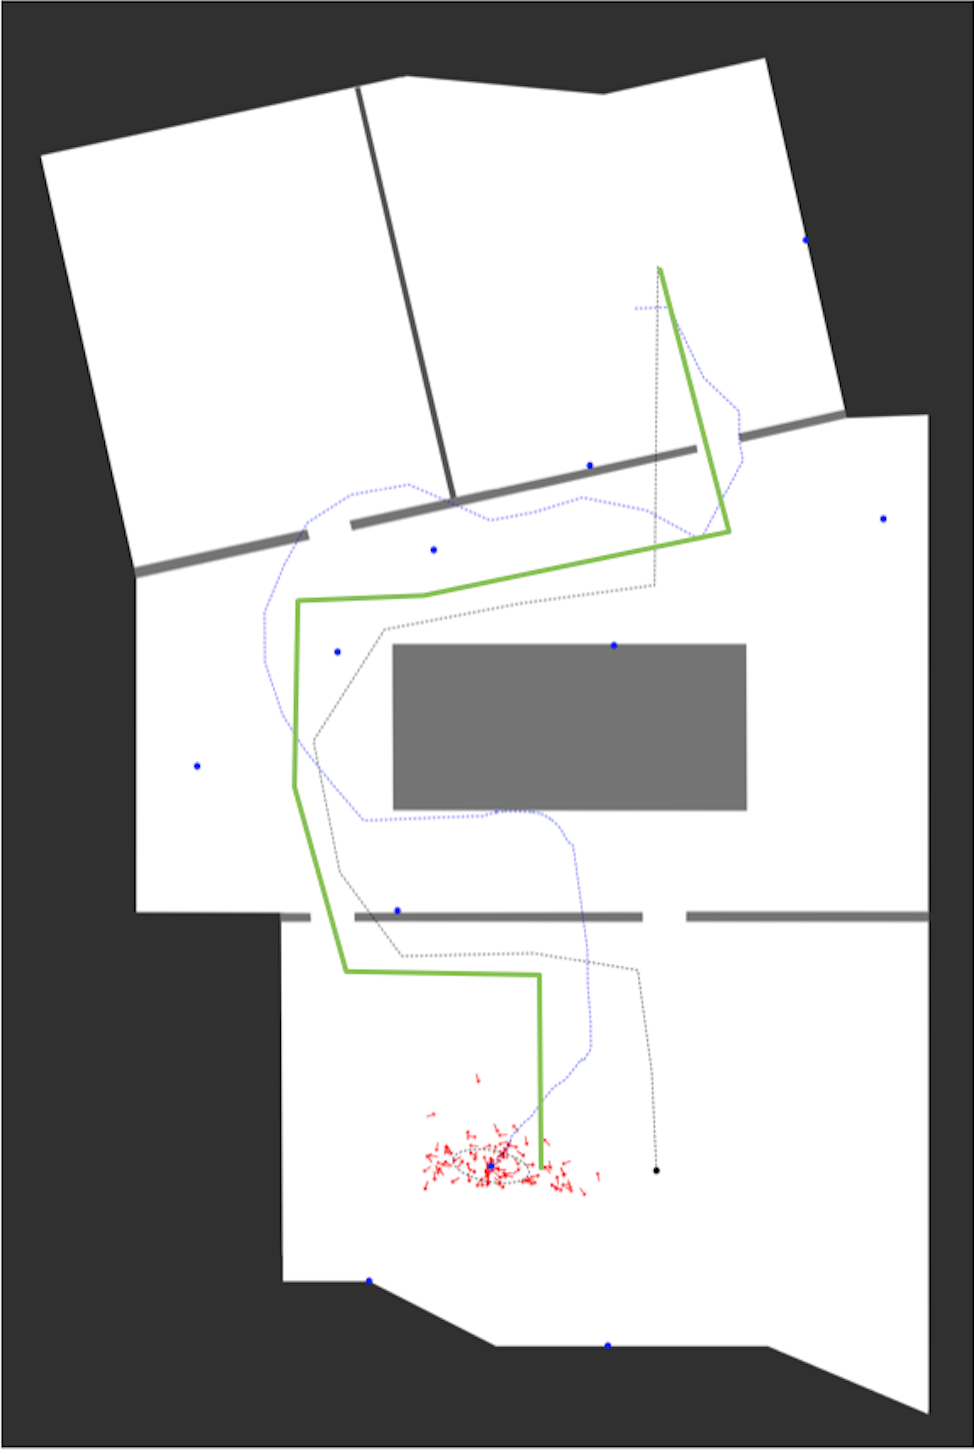
\includegraphics[height=0.45\textheight]{figures/eval_3_1}
  \label{fig:exp3_imgs_1}
}
\subfloat[] {
  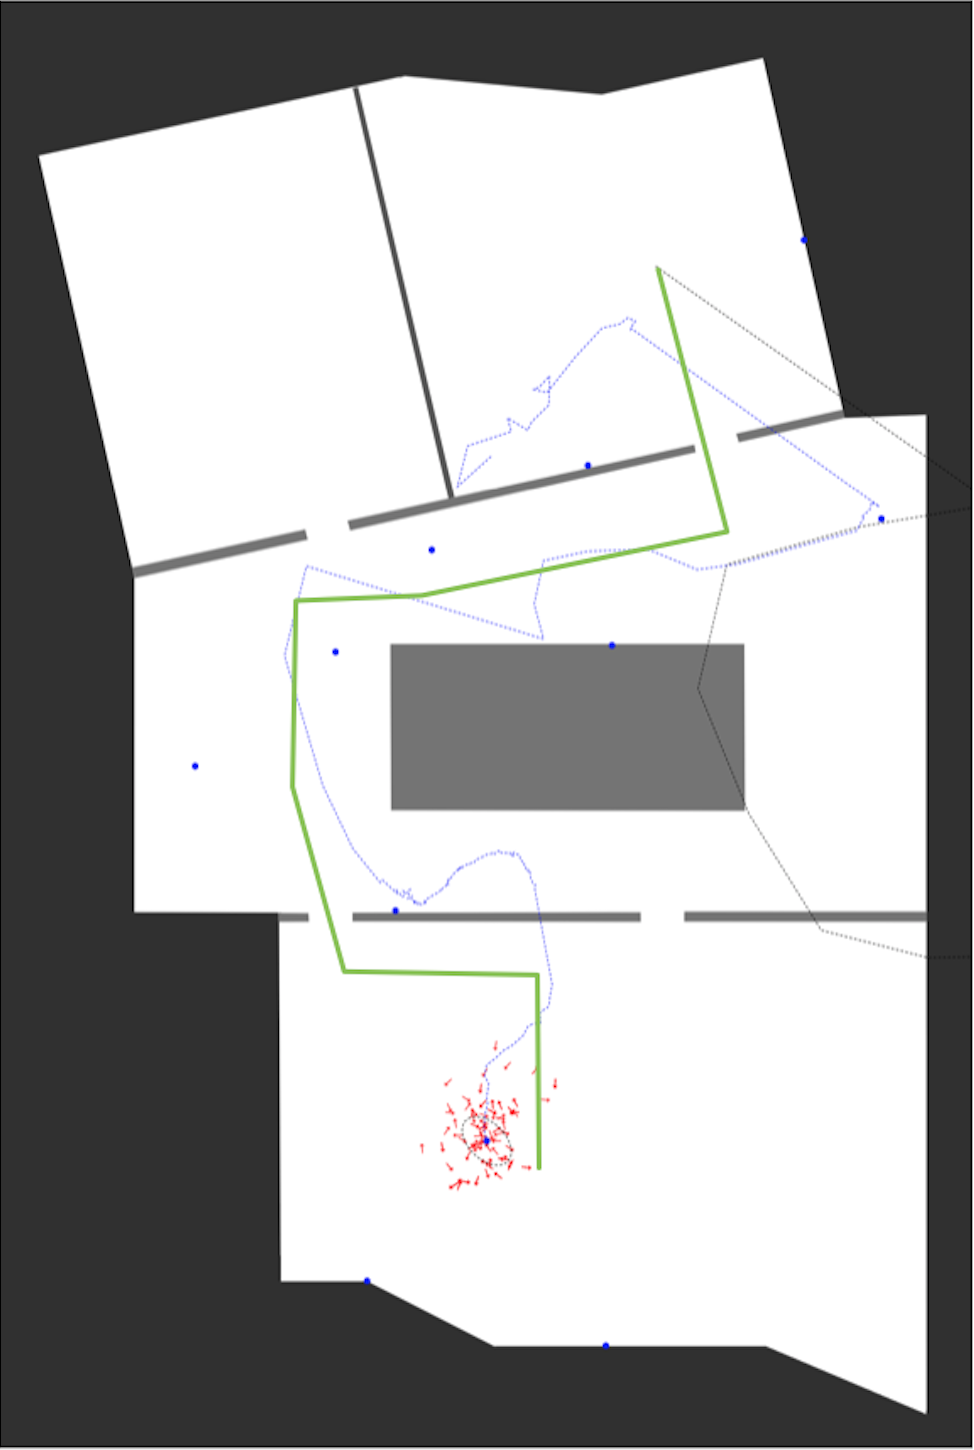
\includegraphics[height=0.45\textheight]{figures/eval_3_2}
  \label{fig:exp3_imgs_2}
}

\subfloat[] {
  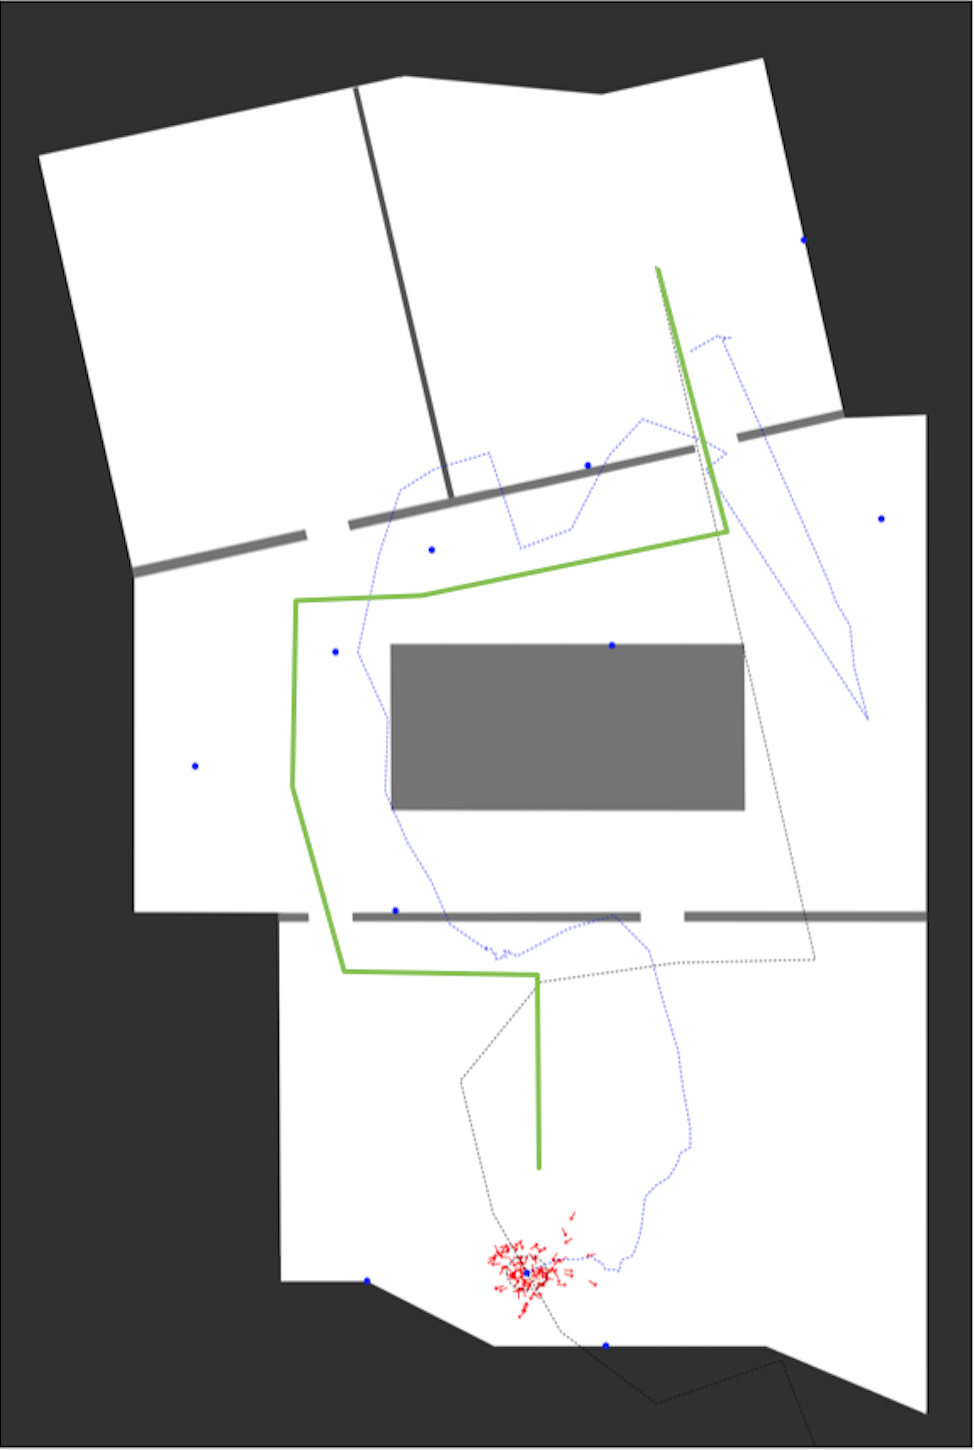
\includegraphics[height=0.45\textheight]{figures/eval_3_3}
  \label{fig:exp3_imgs_3}
}
\subfloat[] {
  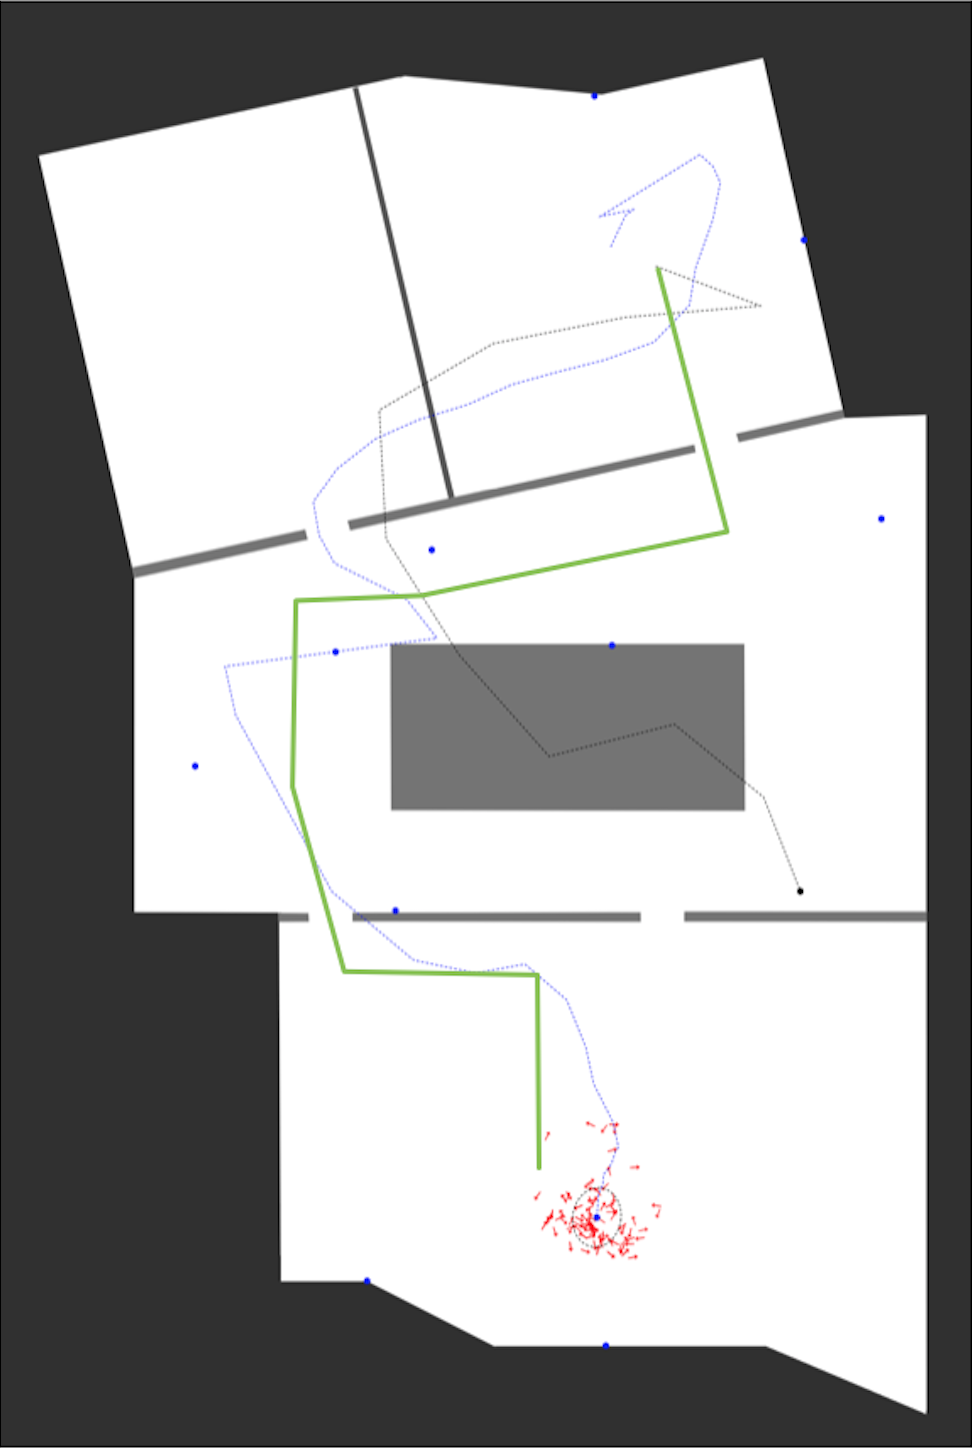
\includegraphics[height=0.45\textheight]{figures/eval_3_4}
  \label{fig:exp3_imgs_4}
}

	\caption{Shows the different beacon deployments during the experiment.}
	\label{fig:exp3_imgs}
\end{figure}

\begin{figure}
	\subfloat[] {
  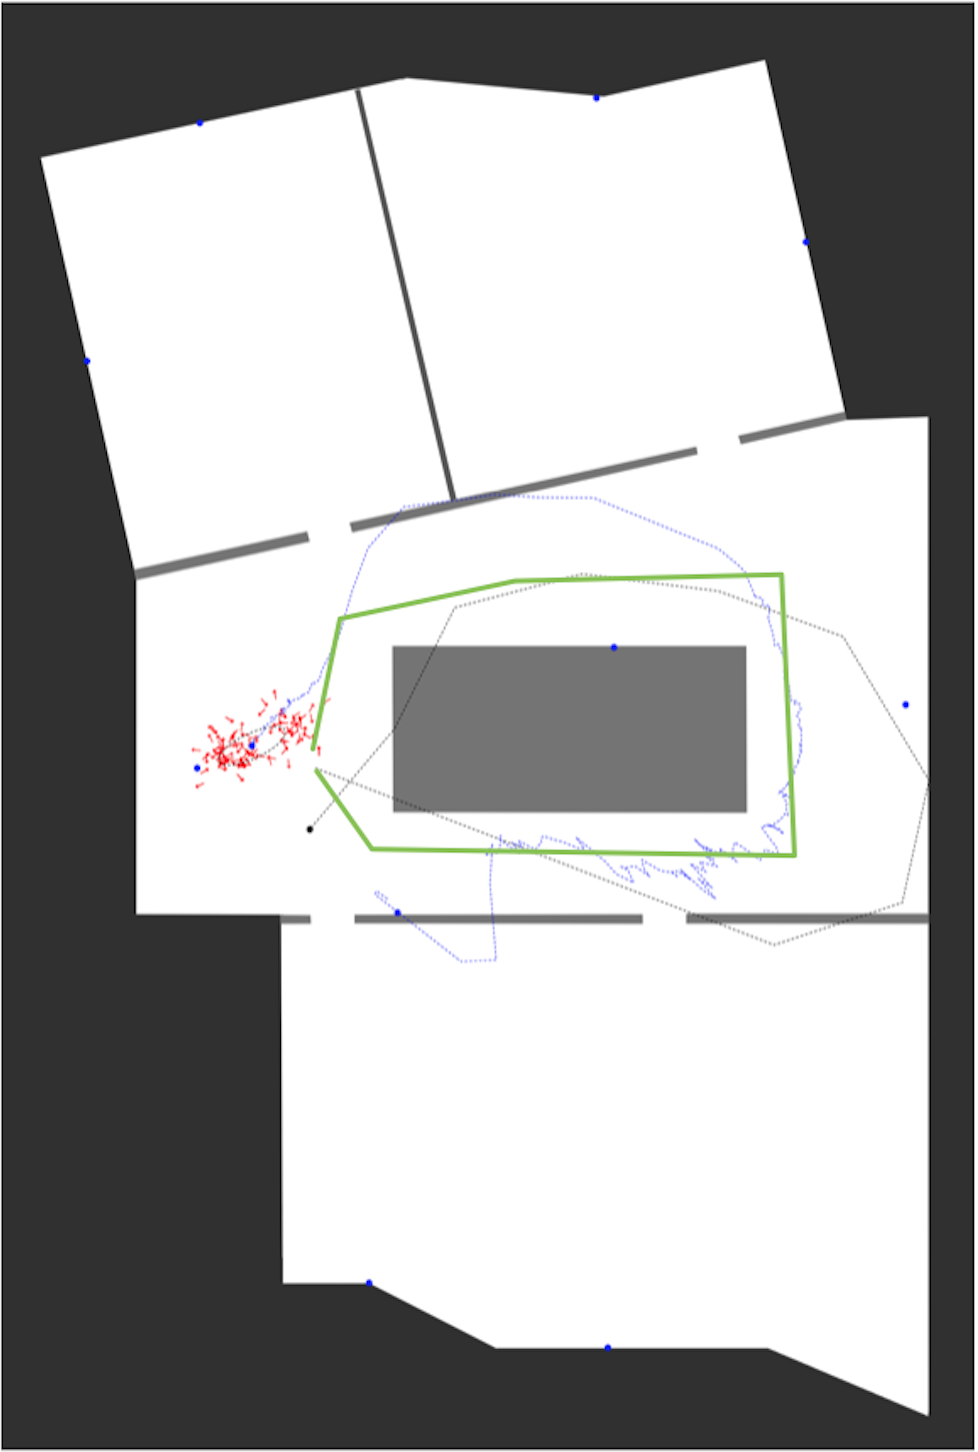
\includegraphics[height=0.45\textheight]{figures/eval_3_5}
  \label{fig:exp3_imgs_5}
}
\subfloat[] {
  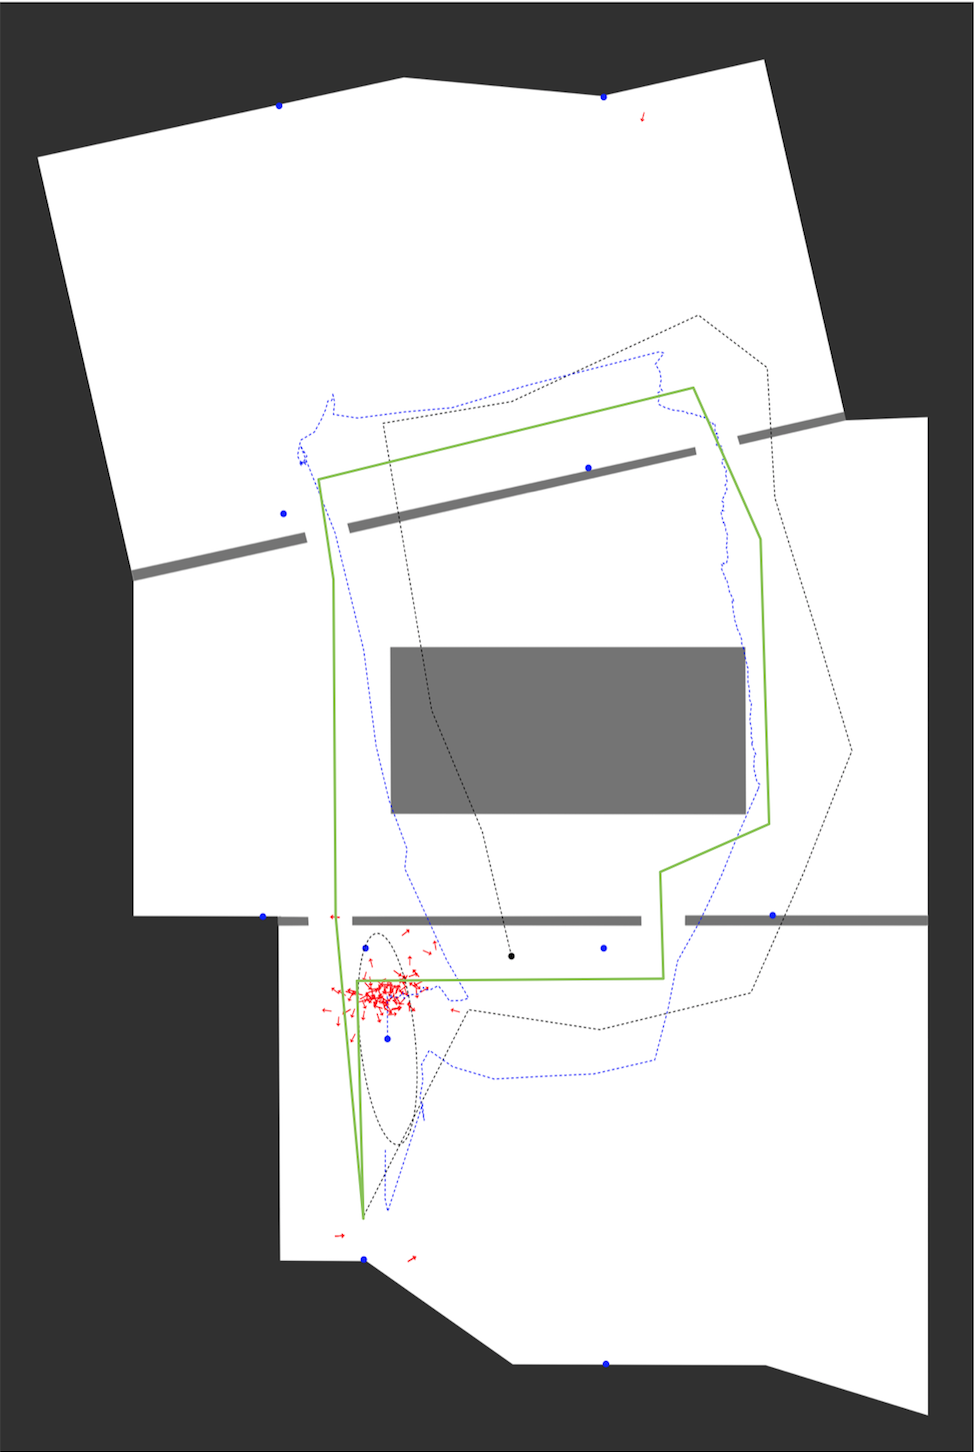
\includegraphics[height=0.45\textheight]{figures/eval_3_6}
  \label{fig:exp3_imgs_6}
}

	\caption{Shows the different beacon deployments during the experiment.}
\end{figure}


\subsection*{Summary}
The algorithm was tested in a typical environment with enabled WiFi, obstacles and many reflecting materials, as shown on the building's images.

The experiments demonstrate that the estimation's accuracy depends on the amount of deployed beacons, but also on their position and attitude relative to the user, which influences the beacons' signals. Furthermore, the experiments showed, that the estimated position not only depends on the beacons' signals. It also depends on the motion's quality. As shown by experiment~3, location estimation is possible with having only a few beacons deployed, but for that the motion must be relatively correct. Besides that it also proves, that if enough beacons are deployed, the solution is able to correct the path on the basis of the beacon's signals.

Furthermore, the experiment's results show, that the location estimation improves after being stationary for a few seconds, if enough beacons are deployed.

Due to the fact that the application's accuracy and precision depend on so many different factors, it is possible to determine, what the system achieved during the experiments. But it is not possible to make a generally valid statement about the system's precision and accuracy. During the experiments it reached an accuracy of up to 1.52\,m (experiment\,2). By combining the results of experiment 1 and 2 (with 10\,beacons), the system reached an accuracy of 2.12\,m ($\mu$\,=\,2.12, $\sigma$\,=\,2.72). The solution's precision, expressed as \ac{CDF}, is shown in figure~\ref{fig:eval:precision}.

To summarize, the solution provides at least room level or even better accuracy, depending on the deployed beacon count and the above mentioned factors. Furthermore, the solution is able to track a user's path in environments with a lot of free space, as shown by the experiments. Consequently, the system's ability to track a user's path in a corridor should be very good, due to the fact that it takes  the map into account. The solution's only disadvantage is, that the user has to hold the device in the hand by pointing it into the user's walking direction. Otherwise the motion's orientation is completely wrong, and thus recovery often needs to be executed.

\pgfmathdeclarefunction{cdf}{2}{%
  \pgfmathparse{1/(1 + exp(-0.07056*((x-#1)/#2)^3 - 1.5976*(x-#1)/#2))}%
}

\begin{figure}
	\begin{tikzpicture}
  \begin{axis}[trim axis left, trim axis right, height=0.4\textheight,
    xlabel={Error / Accuracy $x$ (m)},
    ylabel={$CDF(x)$},
    legend entries={Exp.\ 1, Exp.\ 2, Exp.\ 1+2},
    legend pos=south east,
    grid = major]
    \addplot[red, smooth, mark=no, domain=-6.08:10.66] {cdf(2.29, 2.97)};
    \addplot[blue, smooth, mark=no, domain=-6.08:10.66] {cdf(1.52, 1.79)};
    \addplot[green, smooth, mark=no, domain=-6.08:10.66] {cdf(2.12, 2.72)};
  \end{axis}
\end{tikzpicture}

	\caption{Depicts our solutions precision during the experiments.}
	\label{fig:eval:precision}
\end{figure}


% depends on the beacons position
% on the location in the room
% on the building
% on the beacons itself
% -> on beacons signals, and motion quality

\section{Scalability}
The area covered by the localization system depends only on the provided map and the deployed beacons. Thus, the system is highly scalable. It can be used within a single room. But it also can be extended to a very large, two-dimensional space.

\section{Robustness}
The system is very robust. It can deal with wrong and missing beacon signals, which is a very common problem. Furthermore, it is able to deal with wrong motion data, caused by influenced heading or wrong distance estimations provided by the pedometer, as shown by the experiments.

Due to the implemented recovery, it is also able to detect completely wrong position estimations. The only requirement for the recovery is that the application needs to at least receive the signal from one beacon.

\section{Complexity}
The solution's complexity is relatively low. Besides the beacons and a typical smartphone, no additional infrastructure, such as a network connection or external power supply, is required.
	
Also, the software complexity is relatively low, due to the used \ac{PF} algorithm. Of course, if a platform does not provide such high level \acs{API}'s, especially such as \acl{CM}'s pedometer to estimate the walked distance, this low level of complexity would not be achieved.

\section{Cost}
Besides the beacons no additional infrastructure is required. Furthermore, the users can use their own smartphones. Thus, the building owner just needs to deploy the beacons.

Consequently, the system's cost mainly depends on the area to be covered, and thus on the required amount of beacons and the initial deployment and setup costs. 100\,beacons (incl.\ batteries) from BEACONinside cost 1790EUR, but cheaper manufacturers might exist.

Furthermore, the system's maintenance effort is relatively low. Typically, the beacons' battery lifetime is up to a year or more. And as long as no big changes to the beacons' environment are made, recalibration is not necessary.

\section{Usability}
The localization system is very easy to use. The user just has to download the app from the platform's app store, e.g.\ a chain of store's app. After launching and providing the application access to \acl{BT} the localization can start.

The user interface can be reduced to a minimum by only showing the environments map, the estimated position and the corresponding $1\sigma-\text{ellipse}$, instead of showing the beacons, the motion path, the user's estimated path, and the particle cloud.

There is only one disadvantage from a usability point of view, which is the position estimation's delay. If the user walks the estimated position is only updated ever $\approx$\,3\,s, due to the fact, that \acs{CM} just provides distance estimations every $\approx$\,2.5\,s, as mentioned in chapter~\ref{chap:pf}. If the user is stationary, the delay drops to $\approx$\,1\,s, which is negligible from my point of view.
